\section{Resistive Micromegas}
\label{chap:TPC_sec:micromegas}
Most recent update: 2020-07-24\\
Contact person: Paul Colas (email: paul.colas@cea.fr)\\

\subsection{Introduction}
First Micromegas prototypes were built with a micro-mesh stretched on a frame, and kept on top of
a segmented anode at a fixed distance of \SI{50}{\micro \meter}. The gap is defined by spacers manufactured
by photo-lithographic techniques. Early tests confirmed that, due to ``hodoscope effect'' a resolution
down to \SI{100}{\micro \meter} could not be reached \cite{Arogancia:2007pt}. This triggered studies with charge spreading
developed at Carleton University~\cite{Dixit:2003qg}.
The first resistive material was an AlSi CERMET deposited on a Mylar foil and glued at
\SI{90}{\degreeCelsius} with layer of melting polymer~\cite{2007NIMPA.581..254D}. Later on, a more robust resistive material was
used: the Dupont-de-Nemours Carbon-loaded Kapton.Since 2015, Thin layers of DLC (Diamond-Like Carbon) deposited on Kapton are used as a resistive material. 
Novel way to manufacture the Micromegas detector
were perfected by the Saclay group in partnership with CERN.


\subsection{Recent Milestones}
From 2008 onward, tests with resistive Micromegas were performed in the Large Prototype. From 2008 to 2010
a single module sitting in the middle of the endplate was tested, with dummy modules all around. The 1726 pads, each about \SI{3}{mm} wide
and \SI{7}{mm} long,
were arranged in 24 lines and 72 radial columns, with 2 pads sacrificed to bring the high voltage to the mesh
through the PCB. The standard electronics from the T2K/ND280 neutrino experiment based on the AFTER chip
was used, connected through 20 to \SI{40}{cm} long flat cables~\cite{6418152}.
To minimize the dead area, the so-called ``bulk'' \cite{Giomataris:2004aa} process was used to fix the
mesh on the PCB: in this process a stainless-steal mesh is held by polyimide pillars sandwiching the mesh, melt together
through the mesh. This makes a robust and dust-proof detector, with only \SI{2}
{mm} taken by a grounding ring at the periphery of the module. This ring is used to fix the potential of the resistive anode all around.

Data taken in this 1-module configuration allowed several resistive coatings to be tested. Resistive pastes were discarded, as
their electrical properties were not uniform enough and lead to distortions on the hit position. Carbon-loaded Kapton gave
very good results, with a resolution down to \SI{70}{\micro \meter} at zero drift distance.

Starting in 2011, a completely new integration of the electronics has been carried out to allow the simultaneous operation
of 7 modules. Naked chips were directly wire-bonded on cards. All the protection of the electronics was removed, this functionality
being fulfilled by the resistive coating. The ADC was moved from the front-end to a mezzanine card, all the electronics fitted just behind the module.
At the same time the noise and the power consumption were lowered by 25\%. To connect a module with 1726 channels, only
3 cables need to be connected: a High Voltage cable for the gaseous amplification, a low voltage cable to supply the electronics,
and an optical fiber to transport the data and the command parameters to the mezzanine card.
The production of 9 modules (including 2 spares) and their electronics followed a quasi-industrial scheme.

Data with 7 modules were taken in 2014 and 2015, allowing new topics to be addressed, as module alignment and distortions.
ExB effect induces distortions for tracks reconstructed near the module boundary causing
shifts of almost 1 mm for pad hits located at the extremity of the module.


This is
in agreement with the simulations carried out in the Kolkata group and can be corrected down to \SI{20}{\micro \meter}.

In 2014 and 2015, a two-phase \ce{CO2} cooling was provided to the 7 Micromegas modules. The two-phase coolant, under a pressure of \SI{50}{bar}, circulates at a temperature close to the ambient.
It consists presently of a serpentine running on the back of the modules, in good thermal contact with Aluminum heat sinks, themselves in contact with the chips. The inner pipe diameter is less than a millimeter, giving a moderate contribution to the material budget. The unit
which provides the pressurized \ce{CO2} was funded by KEK and designed by a Nikhef-CERN collaboration.
An efficient cooling was observed for more than 80 hours continuously in 2015 and for 11 days in 2018. In 2019 and 2020 a new Aluminum cooling plate was prototyped using an additive manufacturing technique, with a 2mm diameter serpentine. 

In 2015, two new modules were inserted on the endplate. The resistive material of the new
modules was Diamond-Like Carbon obtained by sputtering on a Kapton foil.
This gives a very robust resistive anode, and the procurement of this material, made in Japan, is more reliable
than the Dupont Carbon-loaded Kapton. These two modules showed identical performance as the other modules.

In 2018, the endplate was equipped with 4 new modules with a DLC anode. Also, a new scheme was applied for the amplification High Voltage : the anode is set at a positive high voltage, and the Micromegas mesh is set to ground, as the surrounding supports. This allows a better field homogeneity near the module boundary and mitigates the distortions. In addition, this improved the operability of the detector : in case of breakdown of one module, its surface remains at ground, leaving the endplate equipotential. 

The dE/dx resolution is shown in Fig.\ref{fig:fig440} as a function of track length. For the ILC TPC size, it is 5\%.
\begin{figure}
\centering
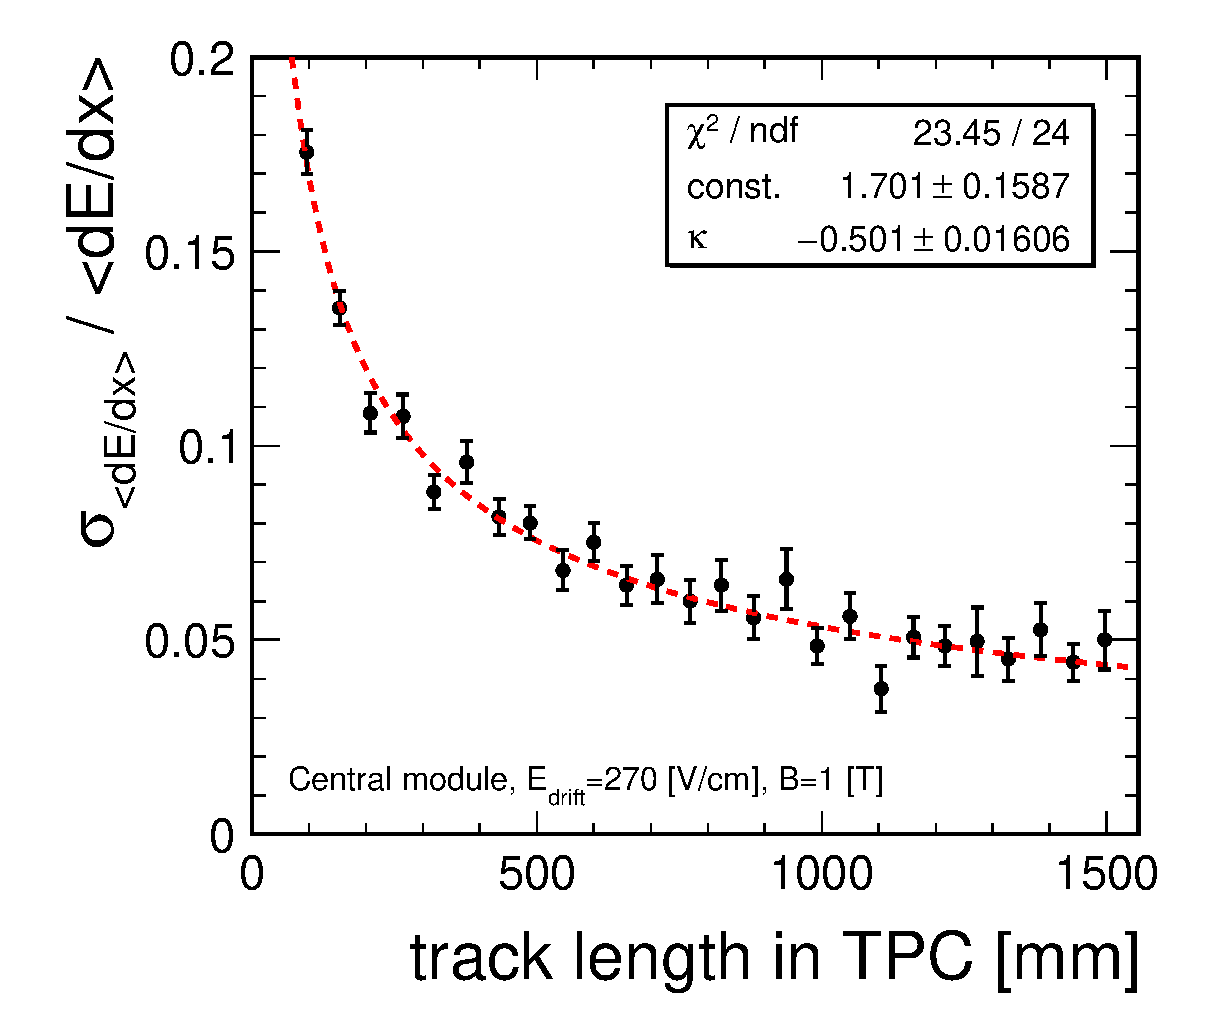
\includegraphics[width=90mm]{Tracker/TPC_Bonn/plots/fig200116_dEdx_modCanvSize.eps}
\caption{The dE/dx resolution as a function of the track length for \SI{5}{GeV} electrons. The red line is a power law.}
\label{fig:fig440}
\end{figure}
The point resolution in the r$\phi$ and z coordinates are shown in Fig.\ref{fig:fig421}. The r$\phi$ resolution reaches \SI{65}{\micro\meter} at zero drift distance, and increases as expected with z, due to electron diffusion during the drift.

\begin{figure}
    \begin{minipage}{0.5\hsize}
        \begin{center}
        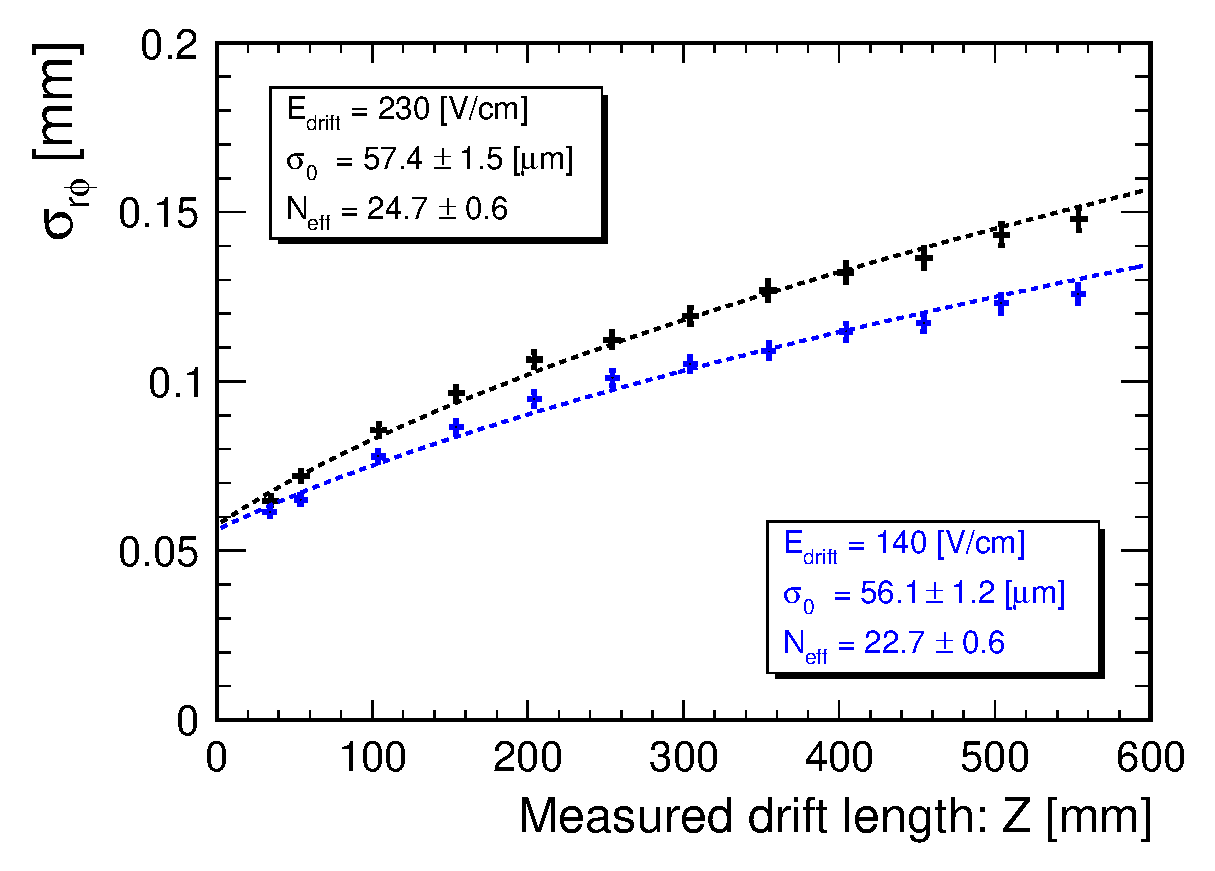
\includegraphics[width=76mm]{Tracker/TPC_Bonn/plots/fig200411_resoX_mod3_24Nov_B1_Ed230Vcm_Ed140Vcm}
        \end{center}
    \end{minipage}
    \begin{minipage}{0.5\hsize}
        \begin{center}
        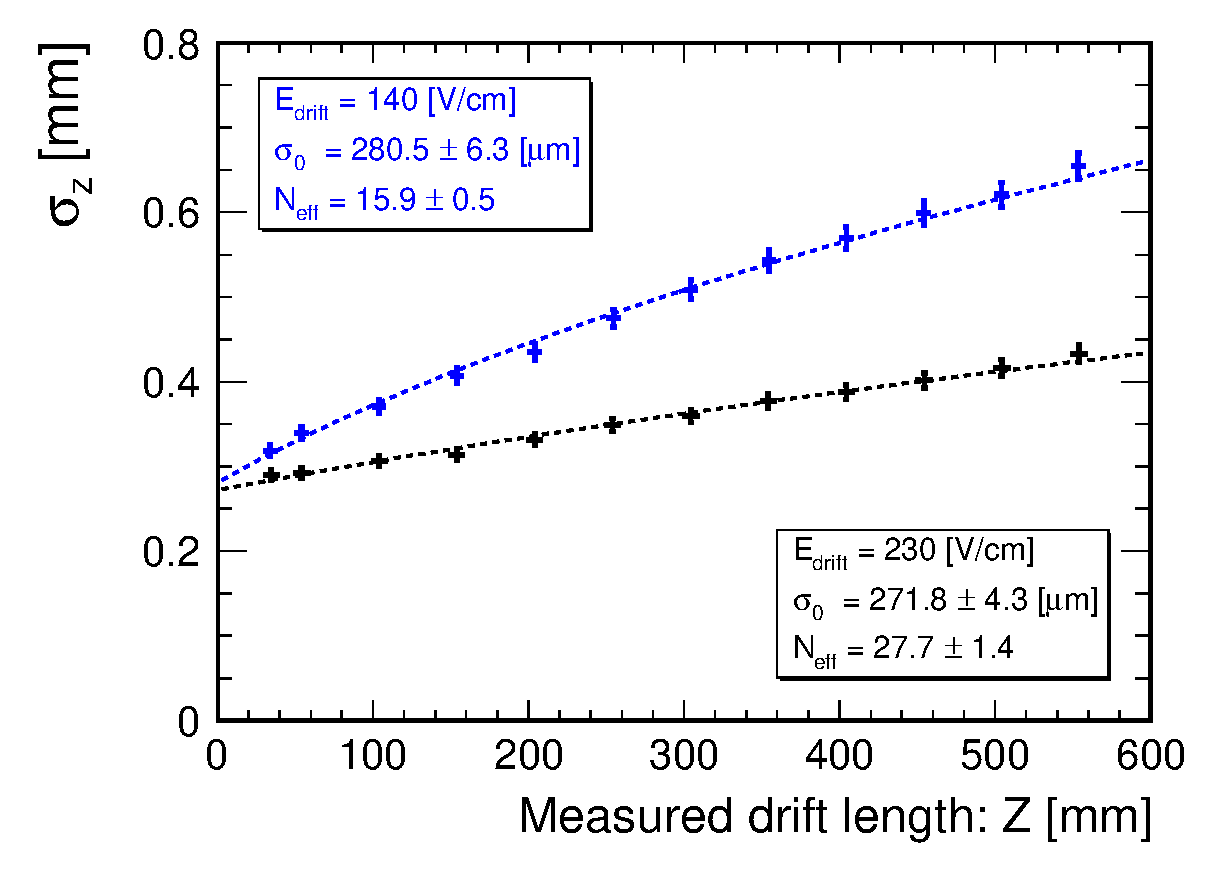
\includegraphics[width=76mm]{Tracker/TPC_Bonn/plots/fig200411_resoZ_mod3_24Nov_B1_Ed230Vcm_Ed140Vcm}
        \end{center}
    \end{minipage}
\caption{The distributions of the spatial and z resolution as a function of the measured drift length, in black for a drift field of \SI{230}{\volt\per\centi\meter} and in blue for \SI{140}{\volt\per\centi\meter} (average over the 24 pad-rows of a module).}
\label{fig:fig421}
\end{figure}


\subsection{Engineering Challenges}
The requirements on the mechanical precision and flatness of the modules are very demanding to keep the systematical errors on the sagitta from distortions below 10-20 microns.

The adaptation of a gating device at a few cm from the end-plate, or integrated to each module, is a
difficult engineering challenge if a minimal degradation of the performances is to be obtained.

The procurement of the DLC is for the time being done from a single Japanese producer. More sources are to be found to secure the supply. Collaboration with RD51 and CERN is in progress on this aspect. 

\subsection{Future Plans}
The time structure of the beams will produce positive ion backflow disks moving slowly (at a few \SI{1}{m/s}) towards the cathode. To experimentally address the question of the effect of these ion disks on the drifting electrons, it is projected to produce such
ions by casting UV light to the cathode for a ms every \SI{100}{ms} or so, while observing distortions on cosmic-ray or beam tracks.
Last but not least, the momentum resolution should be evaluated with long tracks from a particle beam, which requires a silicon
tracker inside the magnet to measure precisely the track position and momentum. For the cooling, further integration work is needed, using micro-channels in the detector board and new material choices for the sink.

In summary, the Micromegas TPC R\&D successfully underwent its proof-of-principle phase and the main integration questions are now addressed. They now request targeted design to progress, thus specific project funding.
